\chapter{Rozszerzenia modelu licencjonowania}\label{chap:extensions}

W niniejszym rozdziale przedstawiono analizę rozszerzeń podstawowego modelu licencjonowania, które uwzględniają różne konfiguracje cenowe oraz ograniczenia pojemności planów grupowych. Badania obejmują osiem wariantów licencyjnych inspirowanych rzeczywistymi ofertami platform takich jak Duolingo, Spotify czy Netflix. Rozdział zawiera szczegółową analizę wpływu poszczególnych parametrów na efektywność optymalizacji oraz porównanie kosztów i czasów wykonania algorytmów w różnych konfiguracjach.

\section{Przegląd badanych wariantów}
Oprócz bazowych konfiguracji rozważono osiem rozszerzeń licencyjnych, które różnią się wielokrotnością kosztu licencji grupowej względem indywidualnej. Warianty Duolingo Super obejmują plany, w których koszt licencji grupowej wynosi odpowiednio dwukrotność, czterokrotność i pięciokrotność ceny licencji indywidualnej, przy zachowaniu stałej pojemności grupy (6 osób). Podobnie, w przypadku dominowania rzymskiego analizowano konfiguracje, w których koszt licencji grupowej wynosi $p$-krotność ceny indywidualnej, dla $p \in \{3, 4, 5\}$. Dwa ostatnie warianty odnoszą się do rzeczywistych ofert: Spotify oferuje plan Duo (pojemność 2) jako wariant pośredni między licencją indywidualną a rodzinną, natomiast Netflix oferuje plany dla 1, 2 lub 4 osób.

Przedstawione w tabelach wartości stanowią statystyki zagregowane dla danej konfiguracji licencyjnej. Oznacza to, że średnie koszty na węzeł oraz średnie czasy obliczeń zostały obliczone na podstawie wyników wszystkich zastosowanych algorytmów oraz wszystkich typów grafów uwzględnionych w eksperymentach. Tabele nie odnoszą się zatem do pojedynczego algorytmu czy sieci, lecz prezentują uśrednione efekty całej grupy uruchomień dla danej konfiguracji licencji.


\subsection{Warianty rodziny Duolingo}
Na rys.~\ref{fig:ext-duolingo-cost} przedstawiono mediany kosztu na węzeł dla konfiguracji, w których koszt licencji grupowej wynosi odpowiednio dwukrotność (\texttt{duolingo\_p\_2}), czterokrotność (\texttt{duolingo\_p\_4}) oraz pięciokrotność (\texttt{duolingo\_p\_5}) ceny licencji indywidualnej. Wyniki wskazują, że wyższe mnożniki prowadzą do wzrostu kosztu na węzeł, co wynika z częstszej selekcji licencji indywidualnych przy wyższych kosztach planów grupowych. W przypadku konfiguracji \texttt{duolingo\_p\_4} oznacza to, że sens kupna licencji grupowej pojawia się dopiero dla grup liczących 4 lub więcej osób, ponieważ dopiero wtedy koszt licencji grupowej jest równy lub niższy niż koszt czterech licencji indywidualnych.

Szczegółowe statystyki dla wariantów Duolingo zebrano w tabeli~\ref{tab:ext-duolingo-stats}. Wzrost mnożnika ceny grupowej z 2 do 5 powoduje wzrost średniego kosztu na węzeł o 77\% (z 0.554 do 0.982) oraz wydłużenie średniego czasu obliczeń o 47\% (z 0.637 s do 0.938 s).

\begin{table}[H]
  \centering
  \caption{Statystyki dla wariantów Duolingo (benchmark statyczny).}
  \label{tab:ext-duolingo-stats}
  \begin{tabular}{llrrrr}
    \toprule
    \textbf{Konfiguracja}   & \textbf{Metryka} & \textbf{Średnia} & \textbf{Odch. std.} & \textbf{Min} & \textbf{Max} \\
    \midrule
    \texttt{duolingo\_p\_2} & Czas [s]         & 0.637            & 1.210               & 0.000        & 7.722        \\
                            & Koszt całkowity  & 49.152           & 39.533              & 8.000        & 177.000      \\
                            & Koszt/węzeł      & 0.554            & 0.152               & 0.340        & 1.000        \\
    \midrule
    \texttt{duolingo\_p\_4} & Czas [s]         & 0.677            & 1.483               & 0.000        & 11.075       \\
                            & Koszt całkowity  & 76.815           & 59.581              & 14.000       & 259.000      \\
                            & Koszt/węzeł      & 0.860            & 0.171               & 0.680        & 1.520        \\
    \midrule
    \texttt{duolingo\_p\_5} & Czas [s]         & 0.938            & 2.721               & 0.000        & 26.589       \\
                            & Koszt całkowity  & 87.855           & 67.852              & 17.000       & 300.000      \\
                            & Koszt/węzeł      & 0.982            & 0.198               & 0.840        & 1.820        \\
    \bottomrule
  \end{tabular}
\end{table}



Analiza rozrzutu wartości w tabeli~\ref{tab:ext-duolingo-stats} pokazuje stabilność wyników. Odchylenie standardowe dla kosztu na węzeł pozostaje na niskim poziomie (0.152--0.198), co wskazuje na konsekwentność rozwiązań algorytmów w różnych instancjach. Warto zauważyć, że w konfiguracji \texttt{duolingo\_p\_5} odnotowano najwyższy maksymalny czas obliczeń (26.589 s), co może wynikać z większej złożoności problemu przy wyższych kosztach planów grupowych. Zwiększone odchylenie standardowe dla czasów wykonania w tej konfiguracji (2.721 s) sugeruje większą wrażliwość algorytmów na charakterystykę konkretnej instancji sieci.

\begin{figure}[H]
  \centering
  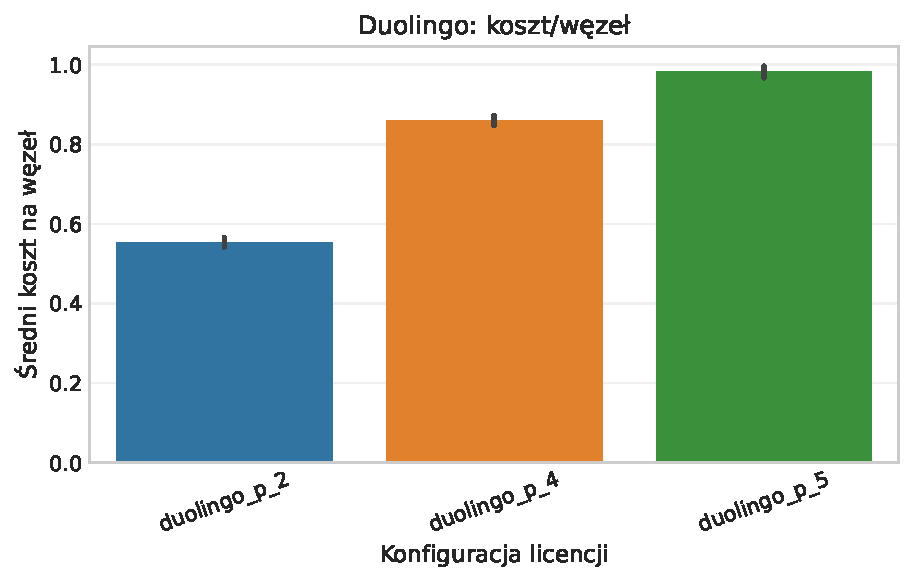
\includegraphics[width=0.6\linewidth]{assets/figures/extensions/static/duolingo_cost_per_node_comparison.pdf}
  \caption{Koszt na węzeł w zależności od planu Duolingo (mediany kluczowych algorytmów).}
  \label{fig:ext-duolingo-cost}
\end{figure}

Zmiana struktury licencji wpływa również na udział planów grupowych. W konfiguracji \texttt{duolingo\_p\_2} ponad połowa przydziałów wykorzystuje licencję grupową, podczas gdy w wariancie \texttt{duolingo\_p\_5} udział grup spada do 24\%, co odzwierciedla rosnący koszt planu grupowego względem licencji indywidualnych.

\subsection{Warianty dominowania rzymskiego}
Na rys.~\ref{fig:ext-roman-cost} przedstawiono mediany kosztu na węzeł dla konfiguracji, w których koszt licencji grupowej wynosi odpowiednio trzykrotność (\texttt{roman\_p\_3}), czterokrotność (\texttt{roman\_p\_4}) oraz pięciokrotność (\texttt{roman\_p\_5}) ceny licencji indywidualnej. Podobnie jak w przypadku planów Duolingo, wyższe mnożniki prowadzą do wzrostu kosztu na węzeł, co wynika z preferencji algorytmów do korzystania z licencji indywidualnych przy wyższych kosztach planów grupowych. Wariant \texttt{roman\_p\_5} charakteryzuje się najwyższym kosztem, co odzwierciedla ograniczoną opłacalność licencji grupowych w tej konfiguracji.

Szczegółowe statystyki dla wariantów dominowania rzymskiego zebrano w tabeli~\ref{tab:ext-roman-stats}. Wzrost mnożnika ceny grupowej z 3 do 5 powoduje wzrost średniego kosztu na węzeł o 37\% (z 0.585 do 0.800) oraz nieznaczne wydłużenie średniego czasu obliczeń (z 0.477 s do 0.493 s).

\begin{table}[H]
  \centering
  \caption{Statystyki dla wariantów dominowania rzymskiego (benchmark statyczny).}
  \label{tab:ext-roman-stats}
  \begin{tabular}{llrrrr}
    \toprule
    \textbf{Konfiguracja} & \textbf{Metryka} & \textbf{Średnia} & \textbf{Odch. std.} & \textbf{Min} & \textbf{Max} \\
    \midrule
    \texttt{roman\_p\_3}  & Czas [s]         & 0.477            & 1.038               & 0.000        & 9.522        \\
                          & Koszt całkowity  & 50.261           & 40.552              & 7.000        & 218.000      \\
                          & Koszt/węzeł      & 0.585            & 0.199               & 0.260        & 1.170        \\
    \midrule
    \texttt{roman\_p\_4}  & Czas [s]         & 0.475            & 1.125               & 0.000        & 9.189        \\
                          & Koszt całkowity  & 60.441           & 48.750              & 9.000        & 259.000      \\
                          & Koszt/węzeł      & 0.701            & 0.232               & 0.340        & 1.400        \\
    \midrule
    \texttt{roman\_p\_5}  & Czas [s]         & 0.493            & 1.289               & 0.000        & 12.314       \\
                          & Koszt całkowity  & 68.995           & 55.987              & 11.000       & 300.000      \\
                          & Koszt/węzeł      & 0.800            & 0.269               & 0.395        & 1.660        \\
    \bottomrule
  \end{tabular}
\end{table}

Zmiana struktury licencji wpływa również na udział planów grupowych (tabela~\ref{tab:ext-license-mix}). W konfiguracji \texttt{roman\_p\_3} udział grup wynosi 43\%, podczas gdy w wariancie \texttt{roman\_p\_5} spada do 24\%. Wyższe koszty planów grupowych prowadzą do preferencji algorytmów w kierunku licencji indywidualnych, co jest zgodne z obserwacjami dla innych rozszerzeń.

\begin{figure}[H]
  \centering
  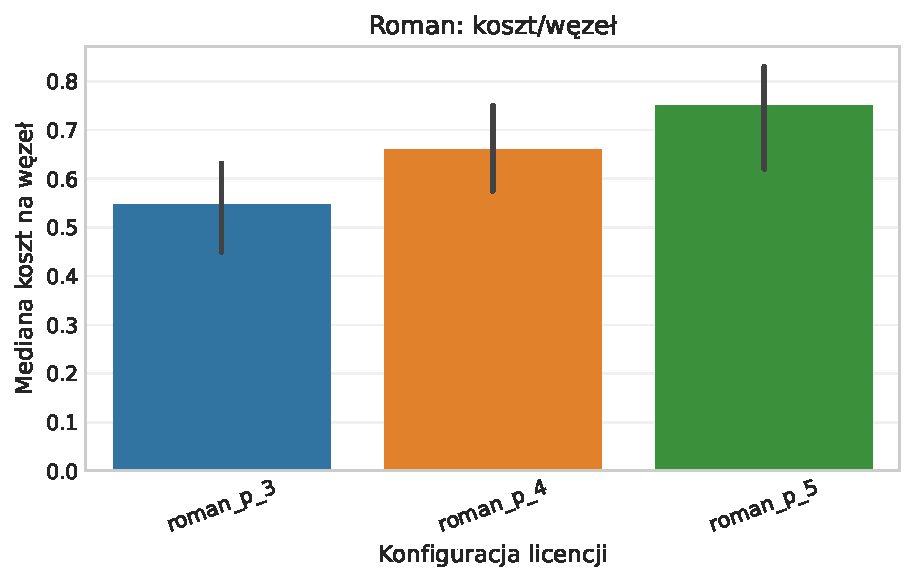
\includegraphics[width=0.6\linewidth]{assets/figures/extensions/static/roman_cost_per_node_comparison.pdf}
  \caption{Koszt na węzeł dla wariantów dominowania rzymskiego.}
  \label{fig:ext-roman-cost}
\end{figure}

\subsection{Spotify i Netflix}

Spotify oferuje plan Duo, przeznaczony dla 2 osób. Umożliwia to efektywne dobieranie użytkowników w pary zamiast tworzenia dużych grup rodzinnych. Tabela~\ref{tab:ext-additional-static} potwierdza, że przeszukiwanie tabu i algorytm genetyczny osiągają najniższe koszty ($0.335$ i $0.400$ na węzeł), uzyskując wyniki niższe niż heurystyka zachłanna.

W przypadku Netflixa plan Standard (również dla 2 osób) stanowi wariant pośredni między licencją indywidualną a planem rodzinnym dla czterech kont, co pozwala metaheurystykom utrzymać koszt w zakresie od $0.60$ do $0.65$ przy czasie poniżej 1~s.

\begin{table}[H]
  \centering
  \caption{Mediany dla konfiguracji Spotify i Netflix.}
  \label{tab:ext-additional-static}
  \begin{tabular}{llrr}
    \toprule
    \textbf{Konfiguracja} & \textbf{Algorytm}   & \textbf{Med. koszt/węzeł} & \textbf{Med. czas [s]} \\
    \midrule
    spotify               & Algorytm zachłanny  & 0.446                     & 0.000                  \\
    spotify               & Algorytm genetyczny & 0.400                     & 0.229                  \\
    spotify               & Algorytm mrówkowy   & 0.391                     & 1.040                  \\
    spotify               & Przeszukiwanie tabu & 0.335                     & 0.958                  \\
    netflix               & Algorytm zachłanny  & 0.682                     & 0.000                  \\
    netflix               & Algorytm genetyczny & 0.650                     & 0.237                  \\
    netflix               & Algorytm mrówkowy   & 0.656                     & 1.289                  \\
    netflix               & Przeszukiwanie tabu & 0.604                     & 0.999                  \\
  \end{tabular}
\end{table}

\begin{figure}[H]
  \centering
  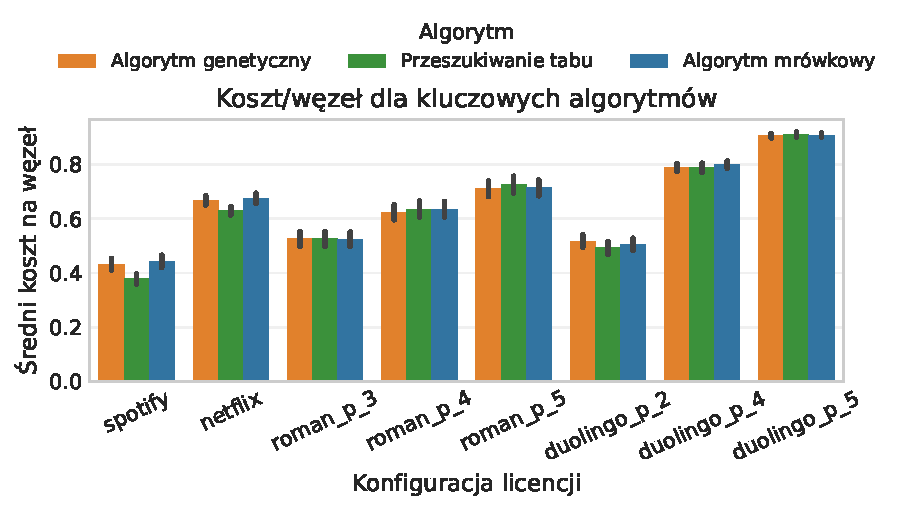
\includegraphics[width=0.6\linewidth]{assets/figures/extensions/static/cost_per_node_by_license_targets.pdf}
  \caption{Koszt na węzeł dla wszystkich rozszerzeń (mediany).}
  \label{fig:ext-license-cost}
\end{figure}


\subsection{Porównanie wszystkich rozszerzeń}

Podstawowe statystyki dla wszystkich konfiguracji zestawiono w tabeli~\ref{tab:ext-overall-static}. W każdym przypadku analizowano ten sam zestaw algorytmów, pomijając obserwacje z przekroczeniem limitu czasu.

\begin{table}[H]
  \centering
  \caption{Statystyki agregowane dla rozszerzeń (benchmark statyczny).}
  \label{tab:ext-overall-static}
  \begin{tabular}{lrr}
    \toprule
    \textbf{Konfiguracja} & \textbf{Śr. koszt/węzeł} & \textbf{Śr. czas [s]} \\
    \midrule
    duolingo\_p\_2        & 0.554                    & 0.637                 \\
    duolingo\_p\_4        & 0.860                    & 0.677                 \\
    duolingo\_p\_5        & 0.982                    & 0.938                 \\
    spotify               & 0.479                    & 0.547                 \\
    netflix               & 0.729                    & 0.623                 \\
    roman\_p\_3           & 0.585                    & 0.477                 \\
    roman\_p\_4           & 0.701                    & 0.475                 \\
    roman\_p\_5           & 0.800                    & 0.493                 \\
  \end{tabular}
\end{table}

Analiza agregowanych statystyk w tabeli~\ref{tab:ext-overall-static} ujawnia wyraźne różnice między rodzinami konfiguracji. W przypadku wariantów Duolingo obserwuje się silną korelację między mnożnikiem ceny grupowej a kosztem na węzeł -- wzrost parametru z 2 do 5 prowadzi do zwiększenia kosztu o 77\% (z 0.554 do 0.982). Jednocześnie czas obliczeń wydłuża się o 47\%, co wskazuje na rosnącą złożoność problemu przy wyższych kosztach planów grupowych.

Warianty dominowania rzymskiego charakteryzują się większą stabilnością obliczeniową, z czasami wykonania w zakresie 0.477--0.493~s niezależnie od parametru $p$. Wzrost kosztu na węzeł jest bardziej umiarkowany (37\% przy wzroście $p$ z 3 do 5), co sugeruje odmienną strukturę przestrzeni rozwiązań w porównaniu z planami Duolingo.

Najkorzystniejszy stosunek kosztu do wydajności obliczeniowej wykazuje konfiguracja Spotify (0.479 kosztu na węzeł przy 0.547~s), co potwierdza skuteczność wprowadzenia planu pośredniego (Duo) między licencjami indywidualnymi a rodzinnymi. Netflix zajmuje pozycję pośrednią z kosztem 0.729 na węzeł, pozostając jednak konkurencyjny pod względem czasu obliczeń (0.623~s).

\subsection{Analiza wpływu liczby użytkowników na koszty}

Struktura wykorzystania licencji zmienia się istotnie (tabela~\ref{tab:ext-license-mix}). W Spotify licencje grupowe odpowiadają za 64\% przydziałów (plan Duo + rodzina), podczas gdy w wariancie \texttt{duolingo\_p\_5} udział grup spada do 24\%. W Netflixie większość przydziałów to plany Standard/Premium (udział 68\%).

\begin{table}[H]
  \centering
  \caption{Udział licencji grupowych i indywidualnych (benchmark statyczny).}
  \label{tab:ext-license-mix}
  \begin{tabular}{lrr}
    \toprule
    \textbf{Konfiguracja} & \textbf{Udział grup} & \textbf{Udział indywidualnych} \\
    \midrule
    duolingo\_p\_2        & 0.56                 & 0.44                           \\
    duolingo\_p\_4        & 0.34                 & 0.66                           \\
    duolingo\_p\_5        & 0.24                 & 0.76                           \\
    spotify               & 0.64                 & 0.36                           \\
    netflix               & 0.68                 & 0.32                           \\
    roman\_p\_3           & 0.43                 & 0.57                           \\
    roman\_p\_4           & 0.34                 & 0.66                           \\
    roman\_p\_5           & 0.24                 & 0.76                           \\
    \bottomrule
  \end{tabular}
\end{table}


\section{Rozszerzenia w środowisku dynamicznym}

W środowisku dynamicznym przeanalizowano te same osiem konfiguracji rozszerzeń, stosując identyczną metodologię jak w benchmarku statycznym. Każda konfiguracja została przetestowana na 272 instancjach dynamicznych, obejmujących różne rozmiary sieci i scenariusze zmian.

\subsection{Statystyki agregowane}

Tabela~\ref{tab:ext-dynamic-family} przedstawia statystyki zagregowane według rodzin konfiguracji. Warianty Duolingo charakteryzują się najwyższymi kosztami średnimi (73.83 na instancję) oraz najdłuższymi czasami wykonania (0.97~s), co wynika z konieczności rozważania licencji o pojemności 6 osób. Problem dominowania rzymskiego wykazuje umiarkowane koszty (59.96) przy porównywalnym czasie obliczeń (0.85~s). Konfiguracje rzeczywistych serwisów -- Spotify i Netflix -- osiągają najkorzystniejsze wyniki, z najniższymi kosztami odpowiednio 43.32 i 66.58.

\begin{table}[H]
  \centering
  \caption{Statystyki zagregowane według rodzin konfiguracji (benchmark dynamiczny).}
  \label{tab:ext-dynamic-family}
  \begin{tabular}{lrrrr}
    \toprule
    \textbf{Rodzina} & \textbf{Śr. czas [s]} & \textbf{Śr. koszt całk.} & \textbf{Śr. koszt/węzeł} & \textbf{Liczba obs.} \\
    \midrule
    Duolingo         & 0.969                 & 73.83                    & 0.792                    & 3265                 \\
    Roman            & 0.853                 & 59.96                    & 0.661                    & 3408                 \\
    Netflix          & 0.891                 & 66.58                    & 0.714                    & 1074                 \\
    Spotify          & 0.881                 & 43.32                    & 0.467                    & 1088                 \\
    \bottomrule
  \end{tabular}
\end{table}

\subsection{Porównanie szczegółowe konfiguracji}

Tabela~\ref{tab:ext-dynamic-detailed} zawiera szczegółowe statystyki dla wszystkich wariantów rozszerzeń. W rodzinie Duolingo obserwuje się wyraźny wzrost kosztu na węzeł wraz ze wzrostem mnożnika ceny grupowej -- od 0.539 w konfiguracji \texttt{duolingo\_p\_2} do 0.980 w \texttt{duolingo\_p\_5}. Podobną tendencję wykazują warianty dominowania rzymskiego, gdzie koszt rośnie z 0.554 (\texttt{roman\_p\_3}) do 0.763 (\texttt{roman\_p\_5}).

\begin{table}[H]
  \centering
  \caption{Szczegółowe statystyki dla rozszerzeń (benchmark dynamiczny).}
  \label{tab:ext-dynamic-detailed}
  \begin{tabular}{lrrrr}
    \toprule
    \textbf{Konfiguracja} & \textbf{Śr. czas [s]} & \textbf{Śr. koszt całk.} & \textbf{Śr. koszt/węzeł} & \textbf{Liczba obs.} \\
    \midrule
    duolingo\_p\_2        & 0.939                 & 50.22                    & 0.539                    & 1088                 \\
    duolingo\_p\_4        & 0.987                 & 80.17                    & 0.855                    & 1073                 \\
    duolingo\_p\_5        & 0.980                 & 90.94                    & 0.980                    & 1104                 \\
    spotify               & 0.881                 & 43.32                    & 0.467                    & 1088                 \\
    netflix               & 0.891                 & 66.58                    & 0.714                    & 1074                 \\
    roman\_p\_3           & 0.798                 & 50.30                    & 0.554                    & 1136                 \\
    roman\_p\_4           & 0.930                 & 60.41                    & 0.666                    & 1136                 \\
    roman\_p\_5           & 0.829                 & 69.18                    & 0.763                    & 1136                 \\
    \bottomrule
  \end{tabular}
\end{table}

Konfiguracja Spotify potwierdza swoją przewagę osiągając najniższy koszt na węzeł (0.467), co stanowi wynik o 13\% lepszy niż w najbliższej konfiguracji \texttt{roman\_p\_3}. Plan Duo umożliwia efektywne parowanie użytkowników, co przekłada się na oszczędności w całym spektrze rozmiarów sieci. Netflix zajmuje pozycję pośrednią z kosztem 0.714 na węzeł, pozostając konkurencyjny wobec wariantów o wysokich mnożnikach.

\subsection{Struktura wykorzystania licencji}

Analiza składu licencji (tabela~\ref{tab:ext-dynamic-license-mix}) ujawnia znaczące różnice w strategiach przydzielania. Konfiguracje o niskich mnożnikach (\texttt{duolingo\_p\_2}, \texttt{spotify}) preferują licencje grupowe, osiągając udział odpowiednio 55\% i 63\%. W przeciwieństwie do tego, wysokie koszty planów grupowych w \texttt{duolingo\_p\_5} i \texttt{roman\_p\_5} prowadzą do dominacji licencji indywidualnych (76\% i 76\% udziału).

\begin{table}[H]
  \centering
  \caption{Struktura wykorzystania licencji (benchmark dynamiczny).}
  \label{tab:ext-dynamic-license-mix}
  \begin{tabular}{lrr}
    \toprule
    \textbf{Konfiguracja} & \textbf{Udział grup [\%]} & \textbf{Udział indywidualnych [\%]} \\
    \midrule
    duolingo\_p\_2        & 55.4                      & 44.6                                \\
    duolingo\_p\_4        & 33.3                      & 66.7                                \\
    duolingo\_p\_5        & 23.0                      & 77.0                                \\
    spotify               & 63.0                      & 37.0                                \\
    netflix               & 66.8                      & 33.2                                \\
    roman\_p\_3           & 41.1                      & 58.9                                \\
    roman\_p\_4           & 33.4                      & 66.6                                \\
    roman\_p\_5           & 23.8                      & 76.2                                \\
    \bottomrule
  \end{tabular}
\end{table}

\begin{figure}[H]
  \centering
  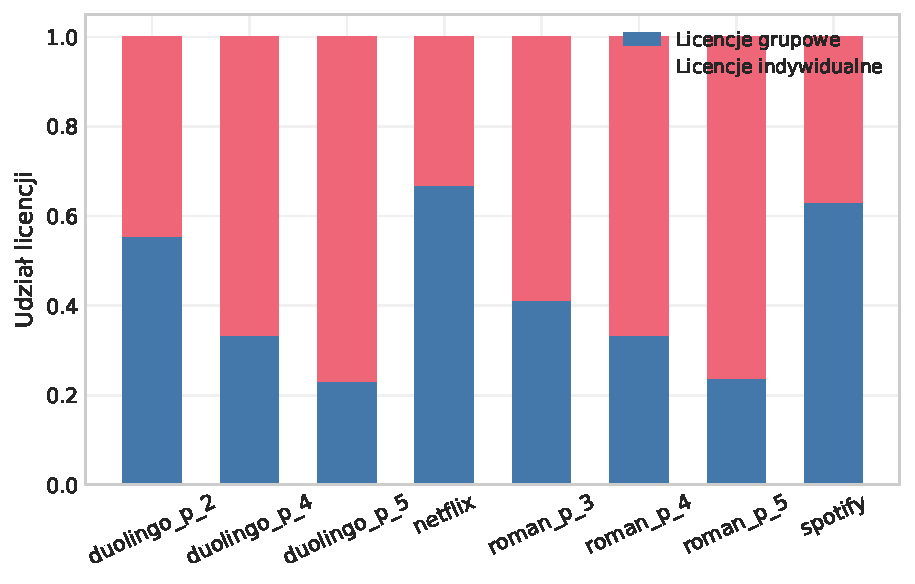
\includegraphics[width=0.8\linewidth]{assets/figures/extensions/dynamic/license_mix.pdf}
  \caption{Udział licencji grupowych i indywidualnych w rozszerzeniach dynamicznych.}
  \label{fig:ext-dynamic-license-mix}
\end{figure}

Netflix wykazuje najwyższy udział planów grupowych (67\%), co wynika z atrakcyjności planów Standard i Premium dla grup 2-4 osobowych. Ta konfiguracja stanowi wariant pośredni między licencjami indywidualnymi a planami o dużej pojemności, umożliwiając algorytmom elastyczne dopasowanie do struktury sieci.

\subsection{Porównanie z benchmarkiem statycznym}

Zestawienie wyników dynamicznych ze statycznymi (tabela~\ref{tab:ext-static-dynamic-comparison}) pokazuje ogólną zgodność trendów. Koszty w środowisku dynamicznym pozostają na podobnym poziomie -- różnice nie przekraczają 3\% dla większości konfiguracji. Czasy wykonania wydłużają się o 30-60\%, co odzwierciedla dodatkową złożoność związaną z dynamicznym rebalansowaniem.

\begin{table}[H]
  \centering
  \caption{Porównanie wyników statycznych i dynamicznych.}
  \label{tab:ext-static-dynamic-comparison}
  \begin{tabular}{lrrrr}
    \toprule
    \textbf{Konfiguracja} & \textbf{Koszt stat.} & \textbf{Koszt dyn.} & \textbf{Czas stat.} & \textbf{Czas dyn.} \\
    \midrule
    duolingo\_p\_2        & 0.554                & 0.539               & 0.637               & 0.939              \\
    duolingo\_p\_4        & 0.860                & 0.855               & 0.677               & 0.987              \\
    duolingo\_p\_5        & 0.982                & 0.980               & 0.938               & 0.980              \\
    spotify               & 0.479                & 0.467               & 0.547               & 0.881              \\
    netflix               & 0.729                & 0.714               & 0.623               & 0.891              \\
    roman\_p\_3           & 0.585                & 0.554               & 0.477               & 0.798              \\
    roman\_p\_4           & 0.701                & 0.666               & 0.475               & 0.930              \\
    roman\_p\_5           & 0.800                & 0.763               & 0.493               & 0.829              \\
    \bottomrule
  \end{tabular}
\end{table}

Najstabilniejsze wyniki wykazuje konfiguracja \texttt{duolingo\_p\_5}, gdzie koszty różnią się jedynie o 0.002 między benchmarkami. Największą poprawę w środowisku dynamicznym odnotowano dla \texttt{roman\_p\_4} (redukcja kosztu o 5\%) i \texttt{roman\_p\_5} (redukcja o 4.6\%). Może to wynikać z lepszego wykorzystania możliwości rebalansowania w mniejszych grupach charakterystycznych dla tych konfiguracji.
\section{Wnioski}

Przeprowadzone badania nad rozszerzeniami modelu licencjonowania pozwoliły na kompleksową analizę wpływu struktury cenowej na optymalizację kosztów w sieciach społecznych. Kluczowe wnioski z analizy ośmiu wariantów licencyjnych można podzielić na trzy główne obszary.

Wpływ mnożnika ceny grupowej na efektywność algorytmów. Badania wykazały wyraźną zależność między stosunkiem ceny licencji grupowej do indywidualnej a skutecznością optymalizacji. W wariantach Duolingo wzrost mnożnika z 2 do 5 powoduje zwiększenie średniego kosztu na węzeł o 77\% (z 0.554 do 0.982) oraz wydłużenie czasu obliczeń o 47\%. Podobną, choć łagodniejszą tendencję obserwuje się w wariantach dominowania rzymskiego, gdzie wzrost parametru $p$ z 3 do 5 prowadzi do 37\% wzrostu kosztu przy stabilnym czasie wykonania. Te wyniki wskazują, że metaheurystyki są najbardziej efektywne przy niskich mnożnikach, gdzie licencje grupowe pozostają opłacalne.

Znaczenie planów pośrednich w strukturze licencji. Analiza konfiguracji rzeczywistych serwisów ujawniła istotną rolę licencji o pojemności pośredniej. Spotify z planem Duo (pojemność 2) osiąga najkorzystniejszy stosunek kosztu do wydajności (0.467 kosztu na węzeł przy 0.547s czasu), podczas gdy Netflix z planem Standard oferuje skuteczne wypełnienie luki między licencjami indywidualnymi a rodzinnymi. W obu przypadkach udział licencji grupowych przekracza 63\%, co potwierdza efektywność elastycznego spektrum opcji licencyjnych.

Stabilność wyników w środowisku dynamicznym. Porównanie benchmarków statycznego i dynamicznego wykazało wysoką zgodność rezultatów -- różnice w kosztach na węzeł nie przekraczają 3\% dla większości konfiguracji. Jednocześnie zaobserwowano wzrost czasów wykonania o 30-60\%, co odzwierciedla dodatkową złożoność związaną z dynamicznym rebalansowaniem. Najstabilniejsze wyniki uzyskano w konfiguracji \texttt{duolingo\_p\_5}, gdzie różnica między środowiskami wynosi jedynie 0.002. Te obserwacje potwierdzają, że proponowane rozszerzenia modelu zachowują skuteczność w realistycznych scenariuszach z czasowymi zmianami struktury sieci.

Otrzymane wyniki mają istotne implikacje praktyczne dla projektowania systemów licencjonowania. Po pierwsze, wprowadzenie planów o pojemności pośredniej może znacząco poprawić efektywność kosztową bez zwiększenia złożoności obliczeniowej. Po drugie, przy wysokich mnożnikach ceny grupowej (powyżej 4-5) korzyści z metaheurystyk maleją, co sugeruje ekonomiczne ograniczenia optymalizacji algorytmicznej. Po trzecie, stabilność wyników w środowisku dynamicznym wskazuje na praktyczną stosowalność proponowanych rozwiązań w rzeczywistych systemach z fluktuacją użytkowników.
